\section{VPN-Typen}
Verschiedene VPN-Typen k�nnen sich z.B. unterscheiden in Protokoll, abstraction layer, access type usw.
VPN's verpacken privat adressierte Pakete in �ffentlich adressierten Paketen. Man nennt das "`tunneling."' Privacy und Authenticity kann durch Verschl�sselungsmechanismen erreicht werden.
\begin{figure}[ht]
	\centering
		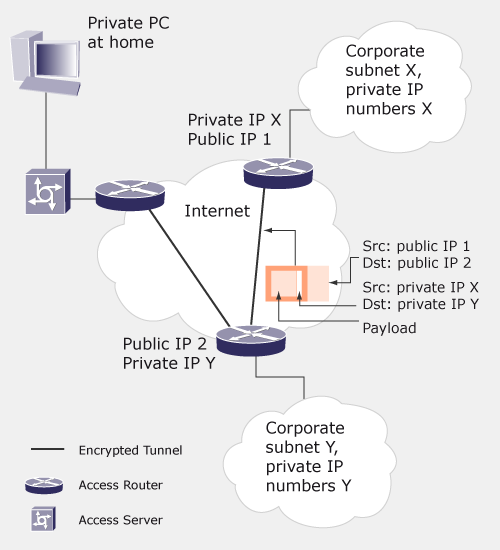
\includegraphics[width=0.50\textwidth]{figure_2_1.png}
		\caption{vpn-types and tunneling}
\end{figure}
\subsection{Subnet-to-Subnet VPN}
Verbindet geographisch getrennte private IP-Subnetzwerke. Der gesamte Datenverkehr, der von einem Subnetzwerk ausgeht und f�r das andere bestimmt ist, wird durch das �ffentliche "`getunnelt."'
\subsection{Access VPN}
 Erm�glicht Roaming-Usern den Zugriff auf das virtuelle Netzwerk von Home-Computern oder �ber einen beliebigen Internet-POP (Point of Presence). Auch hier wird das Tunneling benutzt; entweder �bernimmt ein Home-Computer die Rolle eine Tunnel-Endpunktes, oder der POP eines Internet Service Providers (ISP).